\section{Introduction}\label{sec:introduction}
Le but de cette expérience est de mesurer le coefficient de viscosité $\eta$ de la glycérine
ainsi que de simuler la vitesse de chute d'une bille en fonction du temps dans cette substance
avec les résultats obtenus. \\
Mais tout d'abord, parlons du coefficient de viscosité dans le modèle des forces de la mécanique
de Newton.
La notion de base, c'est qu'une force est une masse multipliée par son accélération :
$\vec{F} = m \cdot \vec{a}$ en $[N]$ dans les unités du système international.
Les différents facteurs de cette définition sont la masse $m$ en $[Kg]$ et l'accélération $a$ en
$\left[\frac{m}{s^{2}}  \right]$, donc la dérivée de la vitesse en $\left[\frac{m}{s}  \right]$
par rapport au temps, et donc la seconde dérivée de la position en $[m]$
($\vec{a} = \dot{\vec{v}} = \ddot{\vec{x}} $), qui dans un cadre expérimental ou autre
ne nécessitant pas un formalisme mathématiques, peuvent être prise comme une
différence pendant un interval de temps ($ v=\frac{\Delta x}{\Delta t} $
et $a = \frac{\Delta v}{\Delta t} $).
Finalement, il faut noter que la somme des forces d'un système est égal à la masse fois l'accélération
totale du système : $\sum\limits_{i}{\vec{F}_{i}} = m \cdot \vec{a}$. \\
Avec ça, il faut donc lister les forces dans le système expérimental (cf.\ figure~\ref{fig:schemaforce}). \\
\begin{minipage}{0.7\textwidth}
    Les trois forces que l'on va prendre en compte sont : la force pesante
    ($F_{p}=m \cdot g $), la force d'Archimède ($F_{a}=\rho_{liquide}
    \cdot V_{immergé} \cdot g $) et la force de frottement du régime laminaire sur une sphère ($F_{f}=
    K \cdot v $ [cas particulier des équations de Navier-Stokes] où $K = 3 \pi D \eta = 6 \pi R \eta $ avec D et R le diamètre et le rayon de la
    sphère ;
    donc $F_{f} =  6 \pi R \cdot \eta \cdot v $).
    Le coefficient de viscosité $\eta$ n'apparait que dans la force de frottement et est mesurée
    en $\left[N \frac{s}{m^{2}}  \right]  = [Pa \cdot s]$ (décapoise), mais en pratique, on privilégie
    le sous-multiple $1 [mPa \cdot s] = 1 \cdot 10^{-3} [Pa \cdot s]$ (centipoise).
    Sachant que la bille est en acier, son volume vaut $\frac{4}{3}\pi R^{3} $ et donc sa masse
    $\frac{4}{3}\pi R^{3} \cdot \rho_{acier} $.
    On considère la vitesse constante (car la vitesse limite est atteinte, voire section \ref{sec:analyse-des-resultats})
    quand on prend la mesure et donc l'accélération nulle.
    En projetant les forces sur un vecteur unitaire de même sens et direction que $\vec{F}_{p} $,
    la somme vectorielle des forces vaut $F_{p}-F_{a}-F_{f}= m \cdot g - \rho_{glycérine}
    \cdot V_{immergé} \cdot g - 6 \pi R \cdot \eta \cdot v = \frac{4}{3}\pi R^{3} \cdot \rho_{acier}
    \cdot g - \rho_{glycérine} \cdot \frac{4}{3}\pi R^{3} \cdot g - 6 \pi R \cdot \eta \cdot v = 0$.
    De fait,
    \[\eta = \frac{\frac{4}{3}\pi R^{3} \cdot \rho_{acier} \cdot g - \rho_{glycérine} \cdot
    \frac{4}{3}\pi R^{3} \cdot g}{6 \pi R  \cdot v} = \frac{2 R^{2} g (\rho_{acier} - \rho_{glycérine})}
    {v} \]
    Les détails concernant la simulation de la vitesse à travers le temps seront évoqués dans la section
    Résultats (\ref{subsec:simulations}).

\end{minipage}
\begin{minipage}{0.05\textwidth}
\end{minipage}
\begin{minipage}{0.25\textwidth}
    \begin{figure}[H]
        \centering
        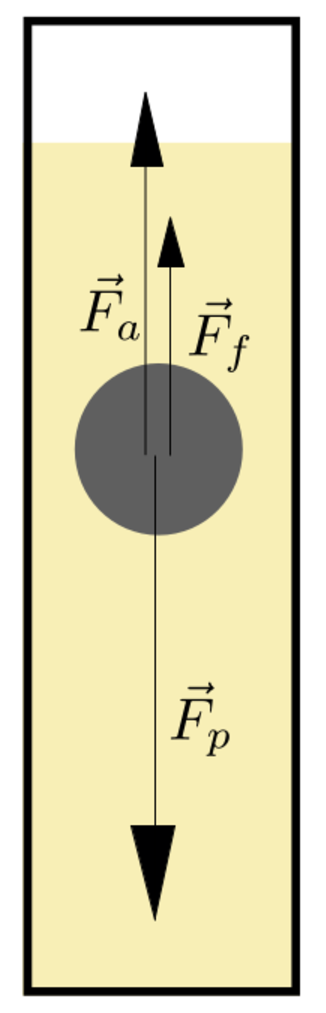
\includegraphics[scale=0.4]{graph/ballinglycsm}
        \caption{Schéma des forces sur une bille dans de la glycérine}
        \label{fig:schemaforce}
    \end{figure}
\end{minipage}